\chapter{Tècniques de segmentació del cos central}
\label{cap:seg}
En aquest capítol s'introdueixen les dues tècniques per a la segmentació del cos central comparades en aquest projecte. La segmentació del cos central bàsicament tracta de trobar la separació entre els ascendents, el cos central i els descendents en una imatge que conté text. Aquesta operació és de vital importància per a diferents tècniques del preprocessament, però sense dubte a la que més afecta és a la normalització de la imatge, que al mateix temps, és una de les etapes del preprocessament que més efecte té sobre la qualitat del reconeixement. \\

Els ascendents i descendents són aquelles parts de la imatge on no resideix molta informació sobre el text representat, mentre que el cos central és aquella part on la major part de la informació resideix. Per exemple, pensem en el cas de les lletres ``o'', ``p'' i ``q''. El que diferència aquestes lletres, és bàsicament la línia vertical que es troba a l'esquerra del cercle, en el cas de la ``p'', i a la dreta, en el cas de la ``q''. Però la longitud d'aquesta línia vertical no aporta massa informació per a diferenciar entre aquestes 3 lletres. Sols és necessari saber si hi ha una línia vertical i on està situada aquesta. Si es traça una línia horitzontal per davall del cercle central de cadascuna de les lletres, aquella part de la imatge que resideix per baix, és el que s'anomenen \emph{descendents}. El mateix passa amb els símbols ``o'', ``b'' i ``d'', però ara la línia vertical es dirigeix cap amunt. En aquest cas, tot el que es troba per damunt del cercle central, serien els \emph{ascendents}. Finalment, en aquest cas, anomenaríem \emph{cos central} al cercle que queda en el centre dels símbols. En la figura \ref{fig:ascendents_descendents_central} hi ha un altre exemple amb les zones diferenciades per a una paraula completa. \\

La línia que separa la zona d'ascendents del cos central s'anomena línia superior i la que separa el cos central dels descendents, inferior o línia base. \\

Una vegada s'ha segmentat el cos central de la imatge (s'han detectat les línies superiors i inferiors), el resultat es pot utilitzar per a normalitzar la grandària dels ascendents i descendents a una porció fixa del cos central, de manera que s'aconsegueix normalitzar l'altura de cadascun dels símbols representats en la imatge aconseguint que el cos central, on resideix la major part de la informació ocupe la major part de la imatge.

\begin{figure}
\centering
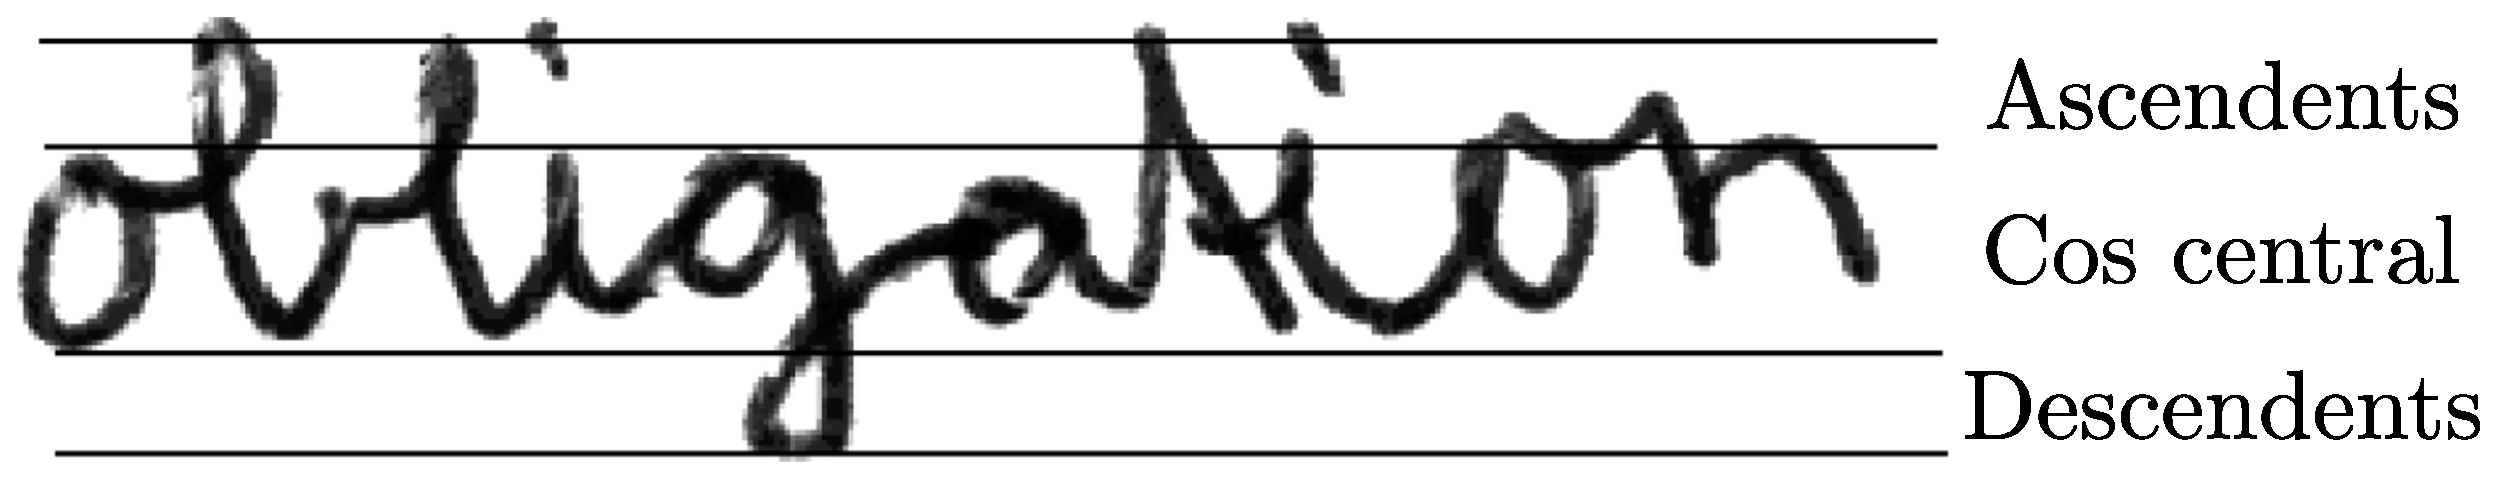
\includegraphics[width=0.8\textwidth]{images/ascendents_descendents_central.eps}
\caption{Zones d'ascendents, cos central i descendents d'una paraula. \cite{Pastor07}}\label{fig:ascendents_descendents_central}
\end{figure}

\section{Aproximació heurística}
\label{sec:seg_heur}
L'algorisme que es descriu en aquesta secció per a detectar el cos central d'una imatge, fou presentat en \cite{Romero05} i \cite{Pastor07} i consisteix en les següents operacions.
\begin{enumerate}
\item La línia es segmenta en diferents parts que estan completament separades per espais blancs. Cadascuna d'aquestes parts serà normalitzada per separat. És important tenir en compte que l'objectiu no és fer un reconeixement del text de cadascuna d'aquestes parts, sinó segmentar el cos central del text en cadascuna d'aquestes parts per separat. Aquesta segmentació de la línia es realitza perquè cada part pot tenir una grandària i forma del cos central diferent.
\item Per a cada part de la línia original, es detecten les línies base i superior de la imatge. Aquesta detecció es subdivideix en els següents passos:
\begin{enumerate}
\item Binarització de la imatge.
\item Suavitzat de la imatge original mitjançant l'algorisme Run-Length Smoothing Algorithm (RLSA).
\item Detecció de les vores superior i inferior de cada segment.
\item Càlcul de les rectes que millor s'ajusten a les fronteres superior i inferior, utilitzant la tècnica dels mínims quadrats.
\end{enumerate}
\end{enumerate}

La figura \ref{fig:pasos_segmentacio_heuristica} mostra tots els passos de la normalització heurística per a una imatge que conté una línia de text de mostra.\\

\begin{figure}
\centering
\begin{subfigure}[b]{0.8\textwidth}
\centering
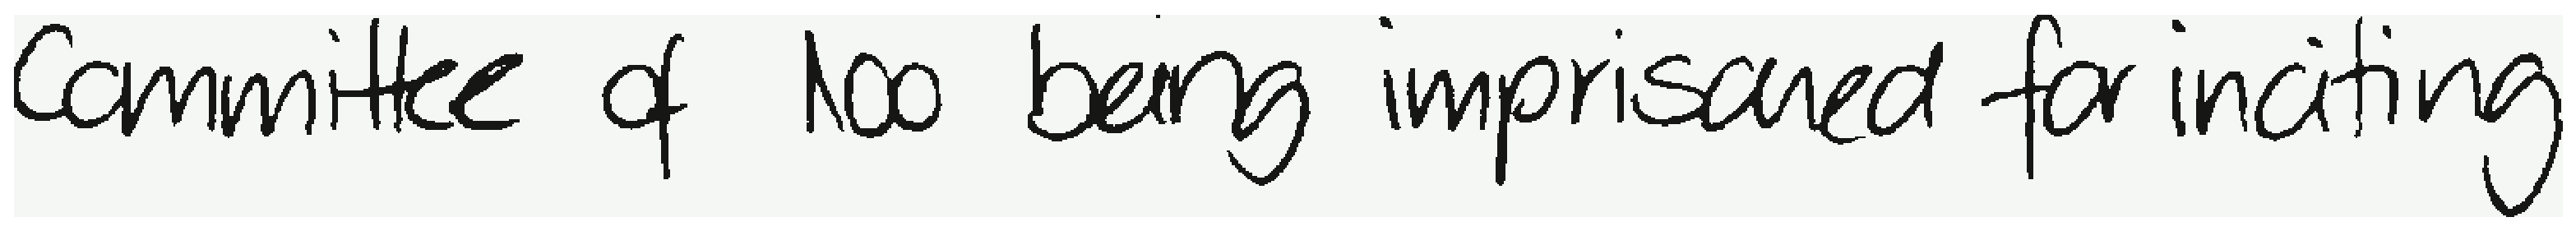
\includegraphics[width=\textwidth]{images/pasos_segmentacio_heuristica_original.eps}
\caption{Imatge original.}\label{fig:pasos_segmentacio_heuristica_original}
\end{subfigure} \\
\begin{subfigure}[b]{0.8\textwidth}
\centering
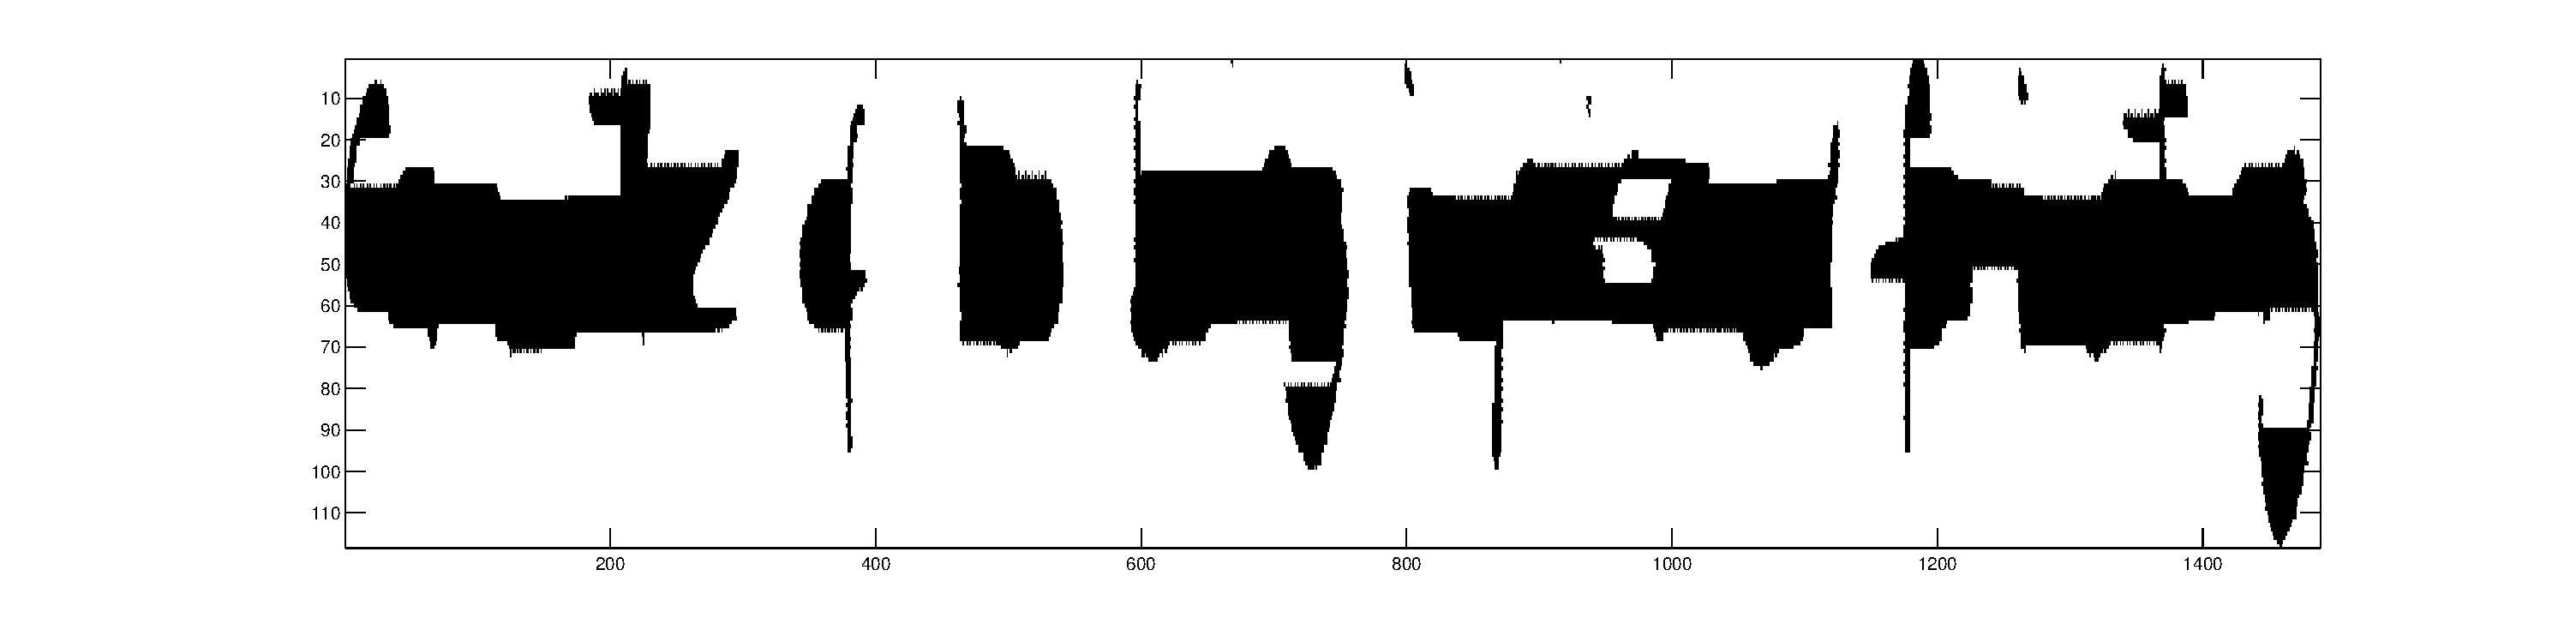
\includegraphics[width=\textwidth]{images/pasos_segmentacio_heuristica_rlsa.eps}
\caption{Resultat de l'algorisme RLSA.}\label{fig:pasos_segmentacio_heuristica_rlsa}
\end{subfigure}\\
\begin{subfigure}[b]{0.8\textwidth}
\centering
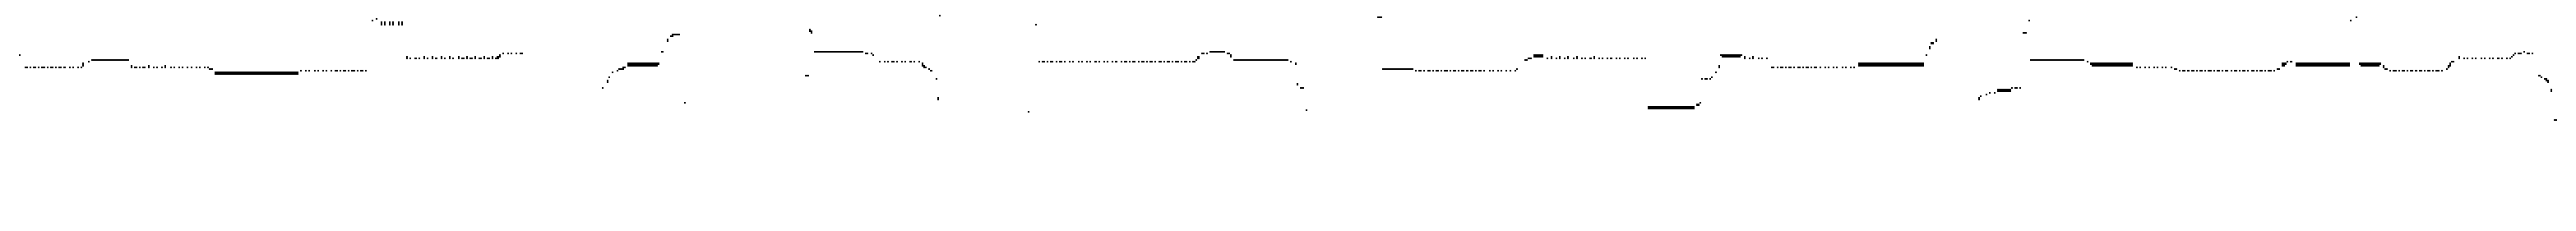
\includegraphics[width=\textwidth]{images/pasos_segmentacio_heuristica_vora_superior.eps}
\caption{Resultat de la detecció de la vora superior.}\label{fig:pasos_segmentacio_heuristica_sup}
\end{subfigure}\\
\begin{subfigure}[b]{0.8\textwidth}
\centering
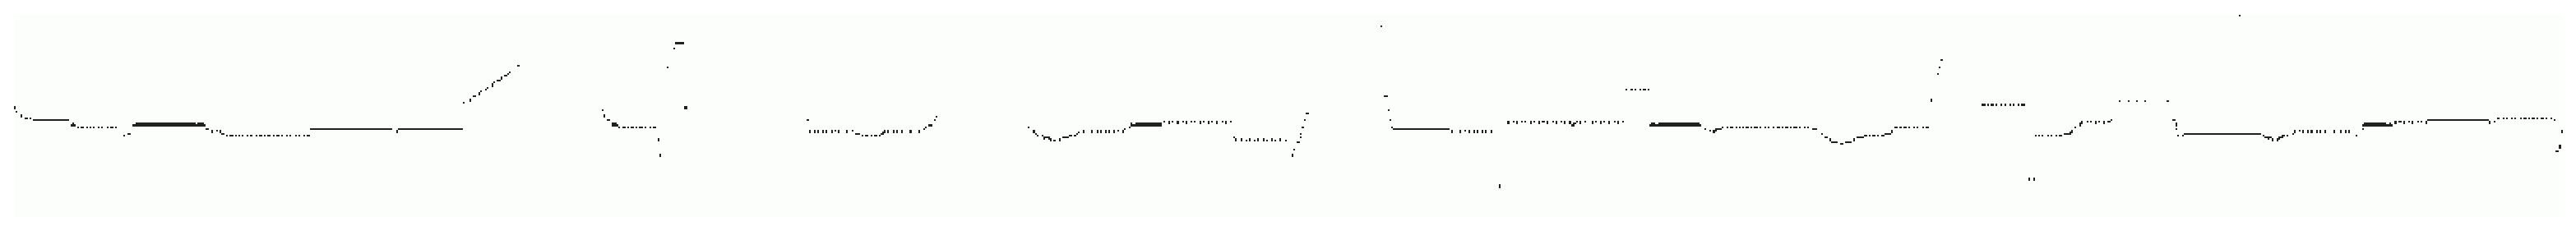
\includegraphics[width=\textwidth]{images/pasos_segmentacio_heuristica_vora_inferior.eps}
\caption{Resultat de la detecció de la vora inferior.}\label{fig:pasos_segmentacio_heuristica_inf}
\end{subfigure}\\
\begin{subfigure}[b]{0.8\textwidth}
\centering
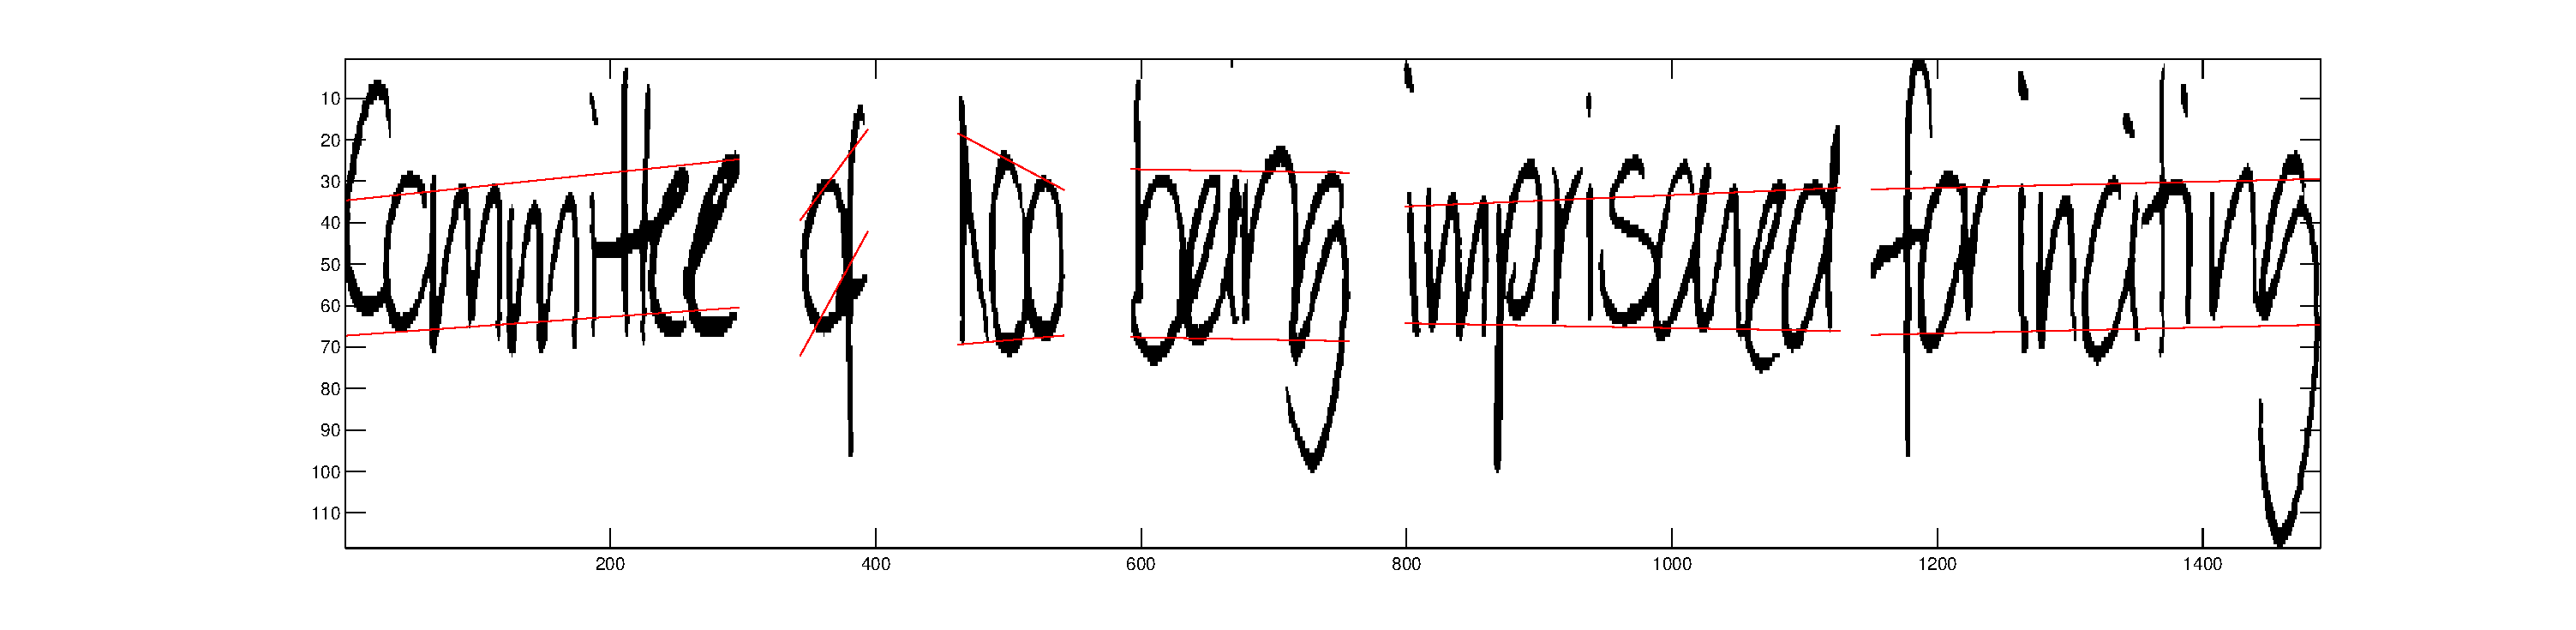
\includegraphics[width=\textwidth]{images/pasos_segmentacio_heuristica_final.eps}
\caption{Resultat final de la segmentació.}\label{fig:pasos_segmentacio_heuristica_final}
\end{subfigure}\\
\caption{Resultat de cada pas de la segmentació del cos central utilitzant l'algorisme heurístic.}\label{fig:pasos_segmentacio_heuristica}
\end{figure}

Aquesta aproximació assumeix que les línies inferiors i superiors poden ser aproximades a una recta amb molt poc d'error. Aquesta assumpció pot no complir-se en la realitat i per tant, pot obtenir una mala aproximació a les línies inferiors i superiors. Un altre inconvenient d'aquest mètode és el llindar que s'utilitza per a fer l'esborronat en l'algorisme RLSA. En aquest algorisme s'uneixen dos píxels negres en una mateixa fila sempre que la separació siga menor que un cert llindar. Aquest llindar pot fer-se fixe o relatiu a la imatge. Siga com siga, si no s'ajusta bé aquest llindar pot ocasionar problemes com els de la figura \ref{fig:pasos_mala_segmentacio}, que alhora fan malbé les diferents etapes del preprocessament que depenen de la segmentació del cos central, com per exemple la normalització de la grandària.

\begin{figure}
\centering
\begin{subfigure}[b]{0.25\textwidth}
\centering
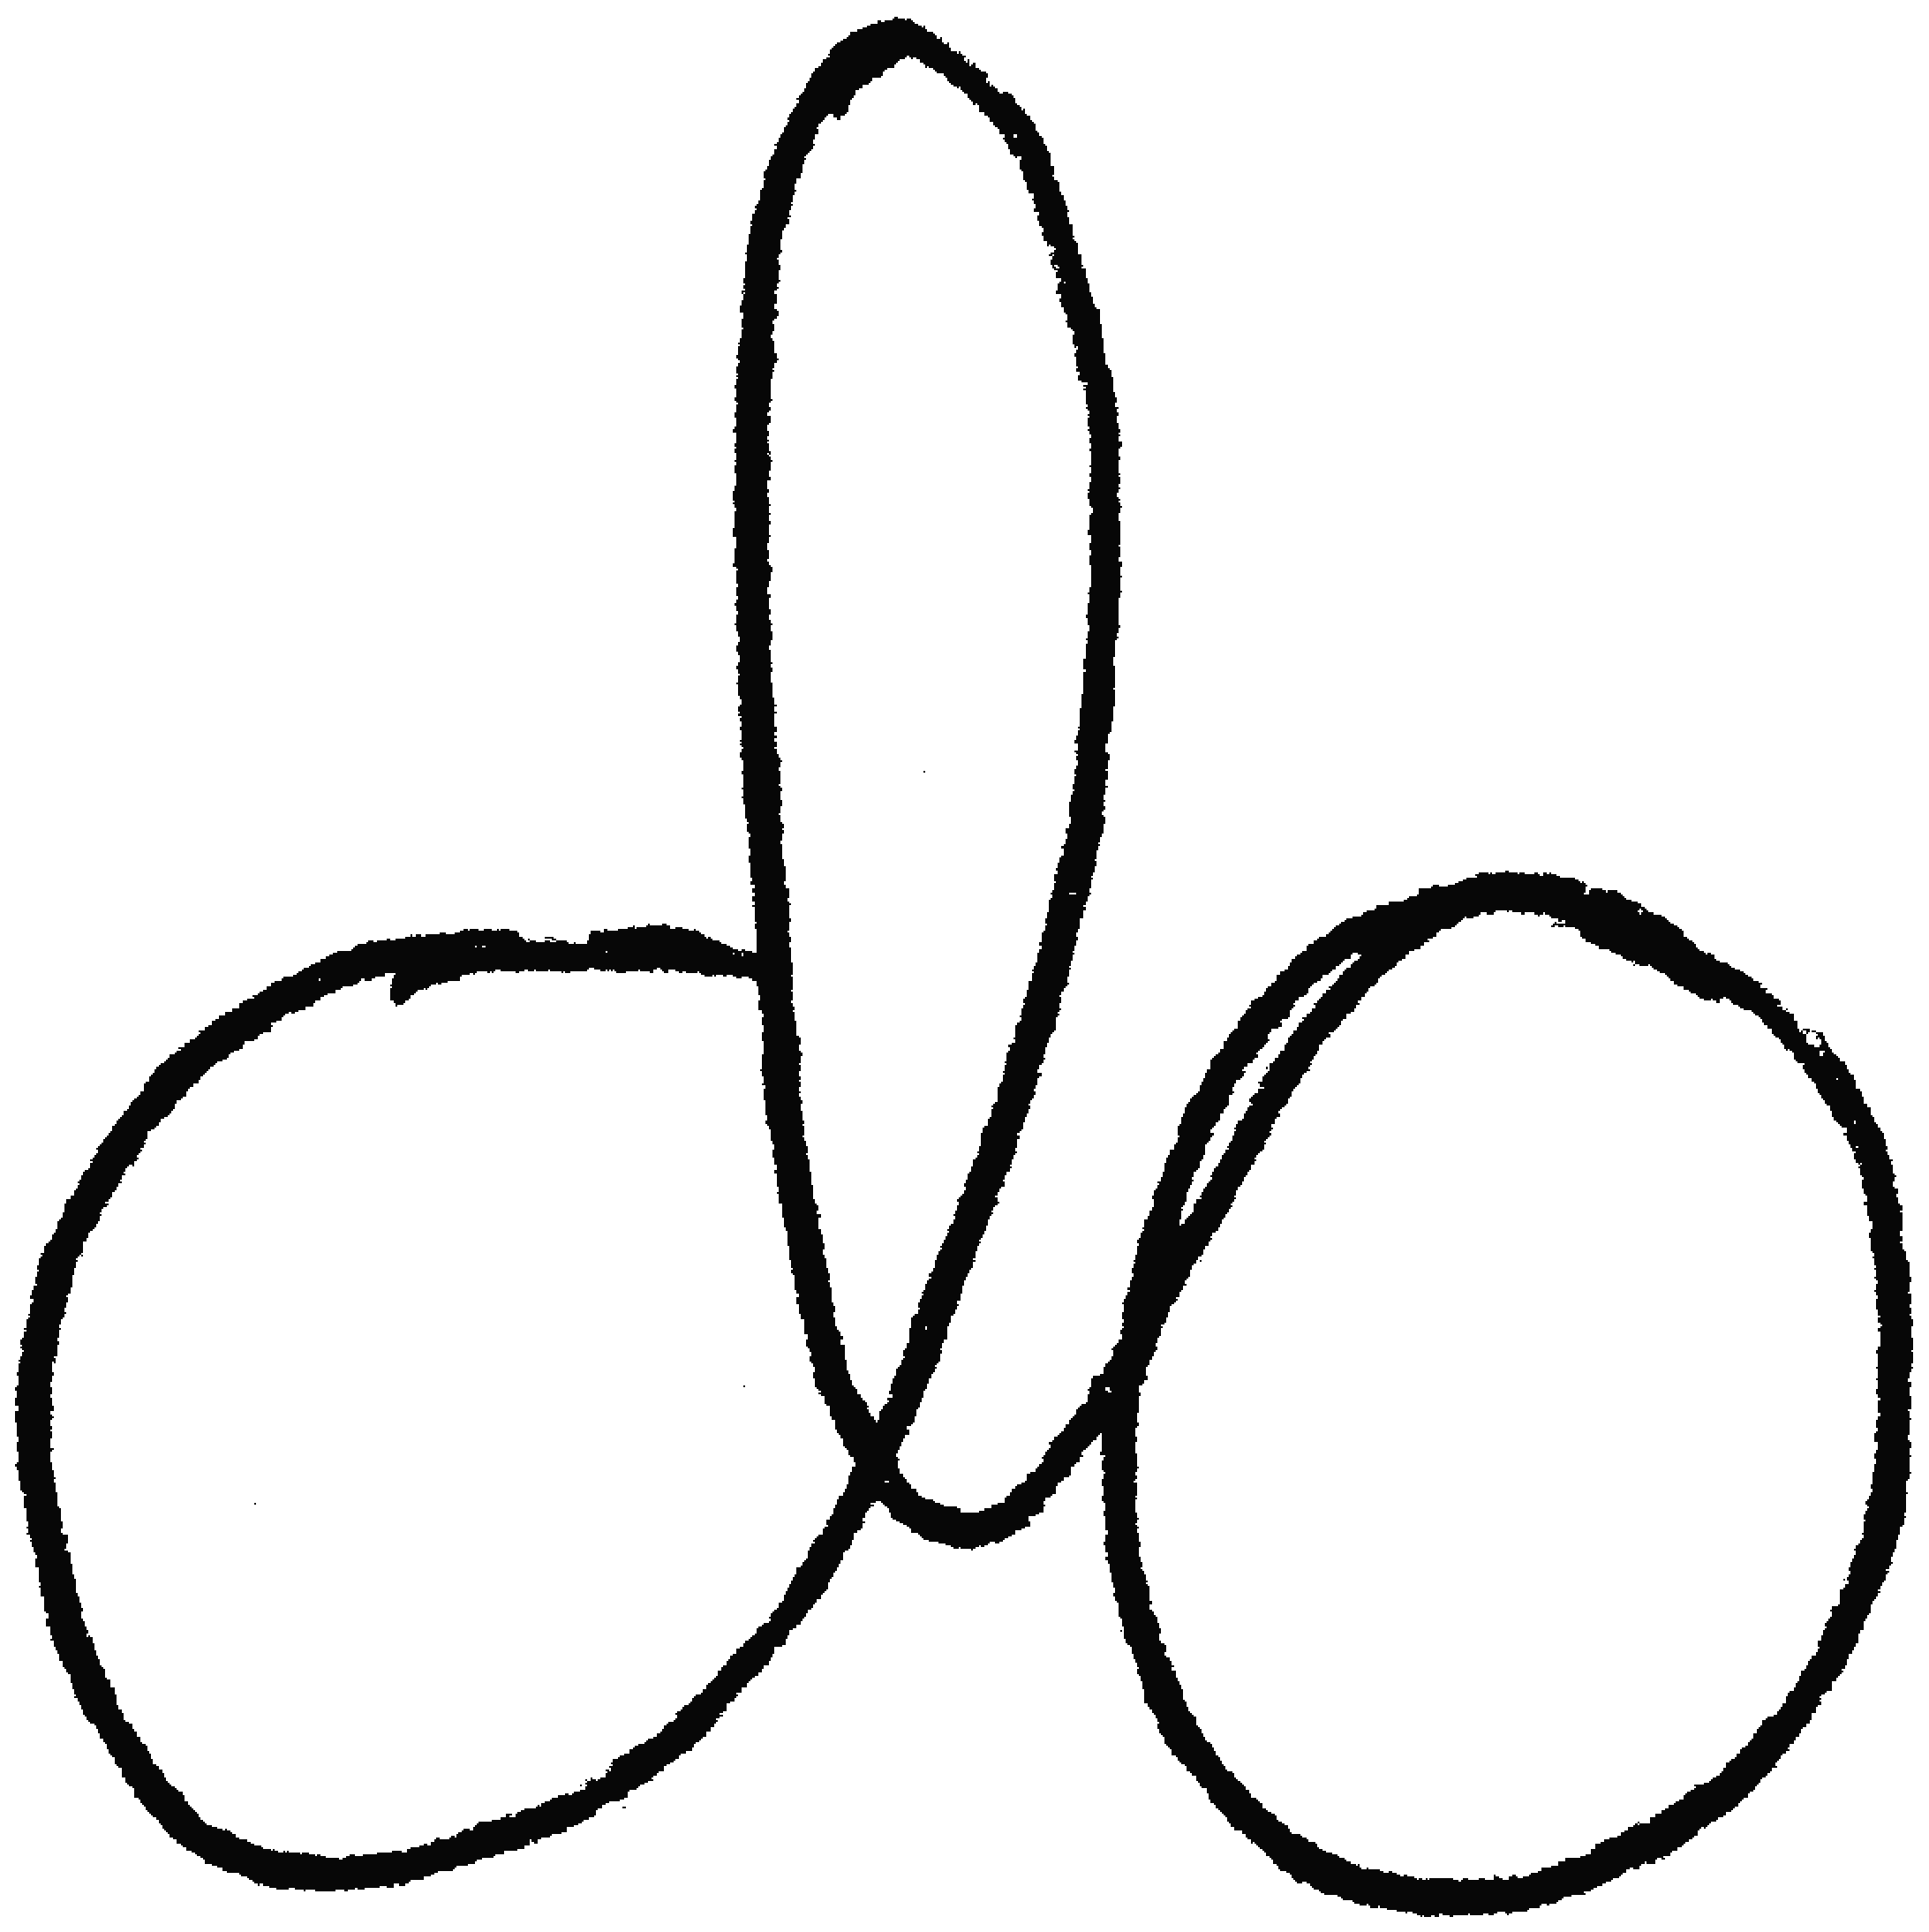
\includegraphics[width=\textwidth]{images/do.eps}
\caption{}\label{fig:pasos_mala_seg_original}
\end{subfigure}
~
\begin{subfigure}[b]{0.25\textwidth}
\centering
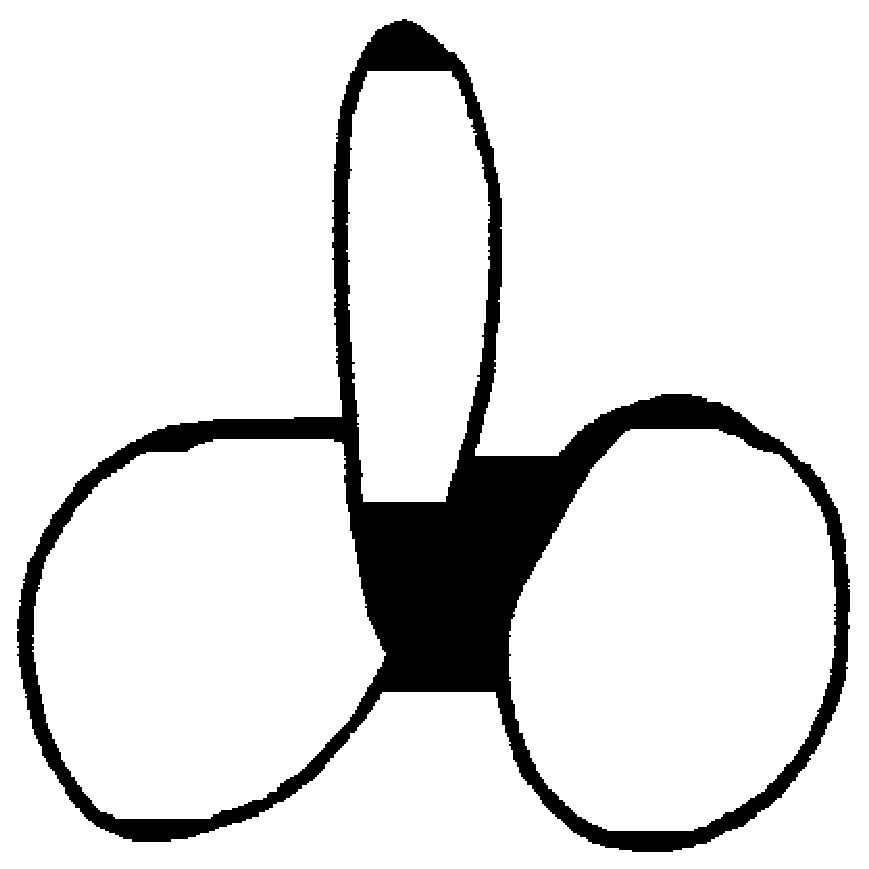
\includegraphics[width=\textwidth]{images/do_RLSA.eps}
\caption{}\label{fig:pasos_mala_seg_rlsa}
\end{subfigure}
~
\begin{subfigure}[b]{0.25\textwidth}
\centering
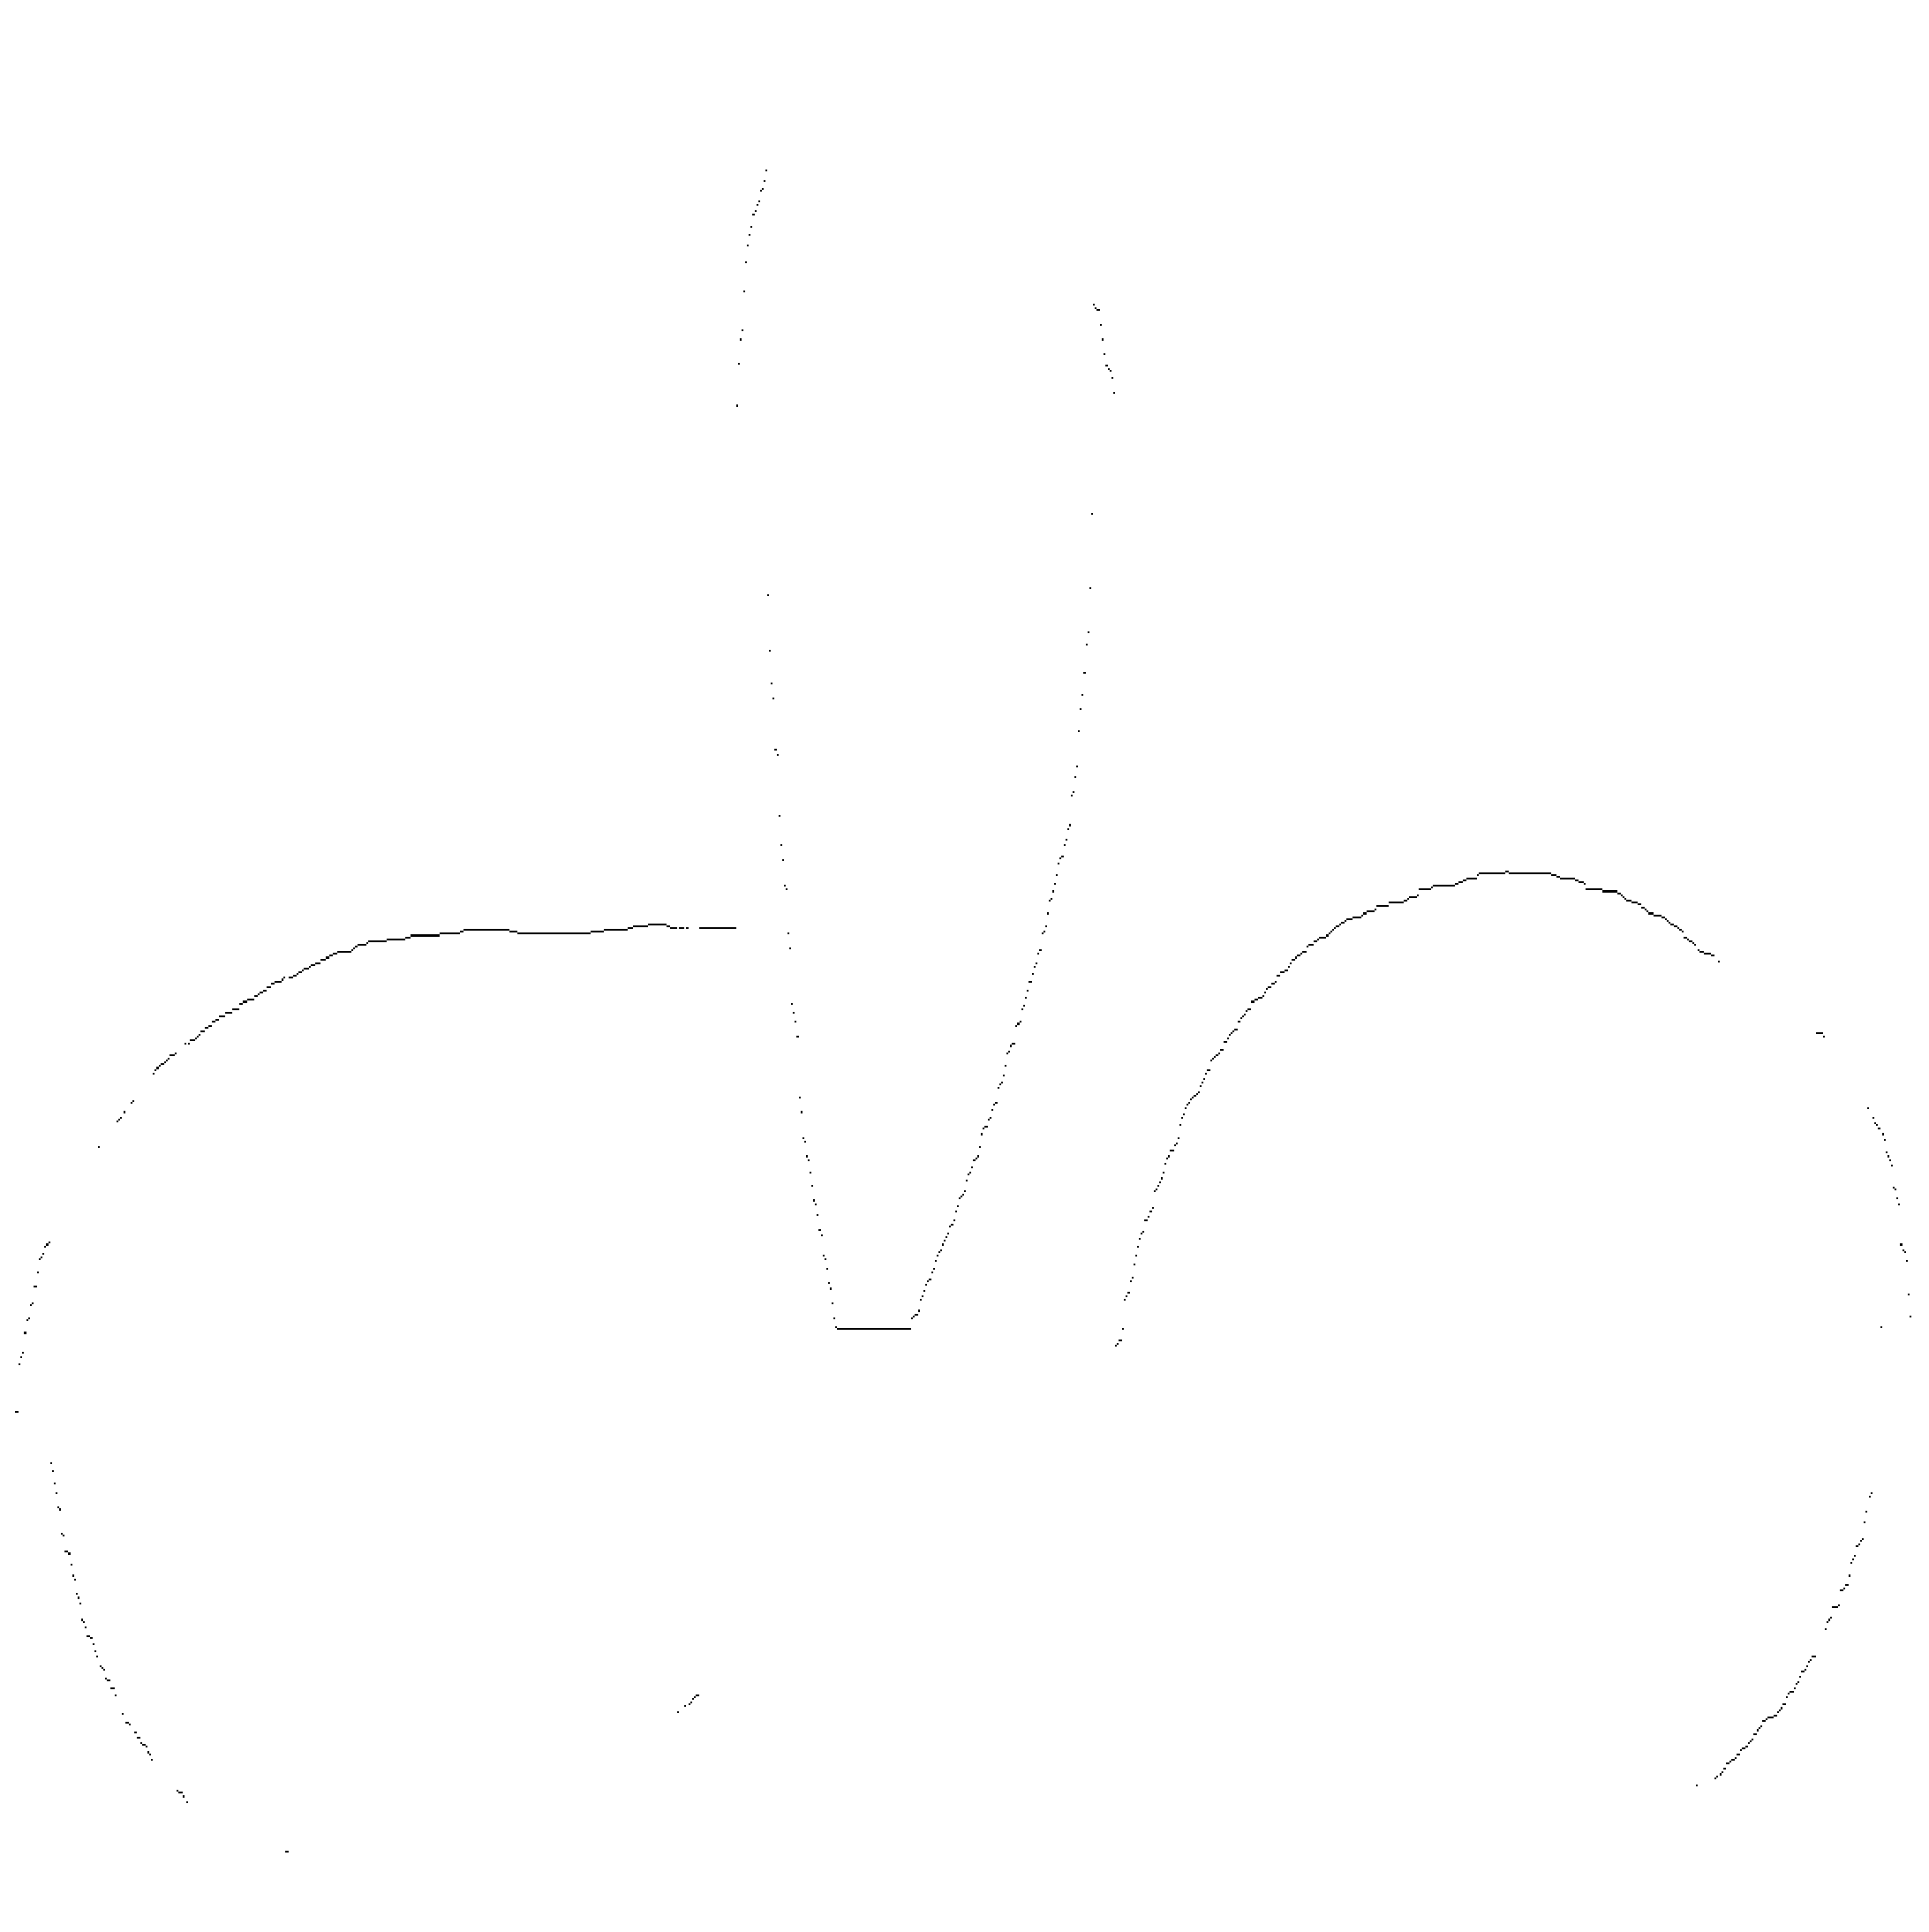
\includegraphics[width=\textwidth]{images/do_upcont.eps}
\caption{}\label{fig:pasos_mala_seg_sup}
\end{subfigure}\\
\begin{subfigure}[b]{0.25\textwidth}
\centering
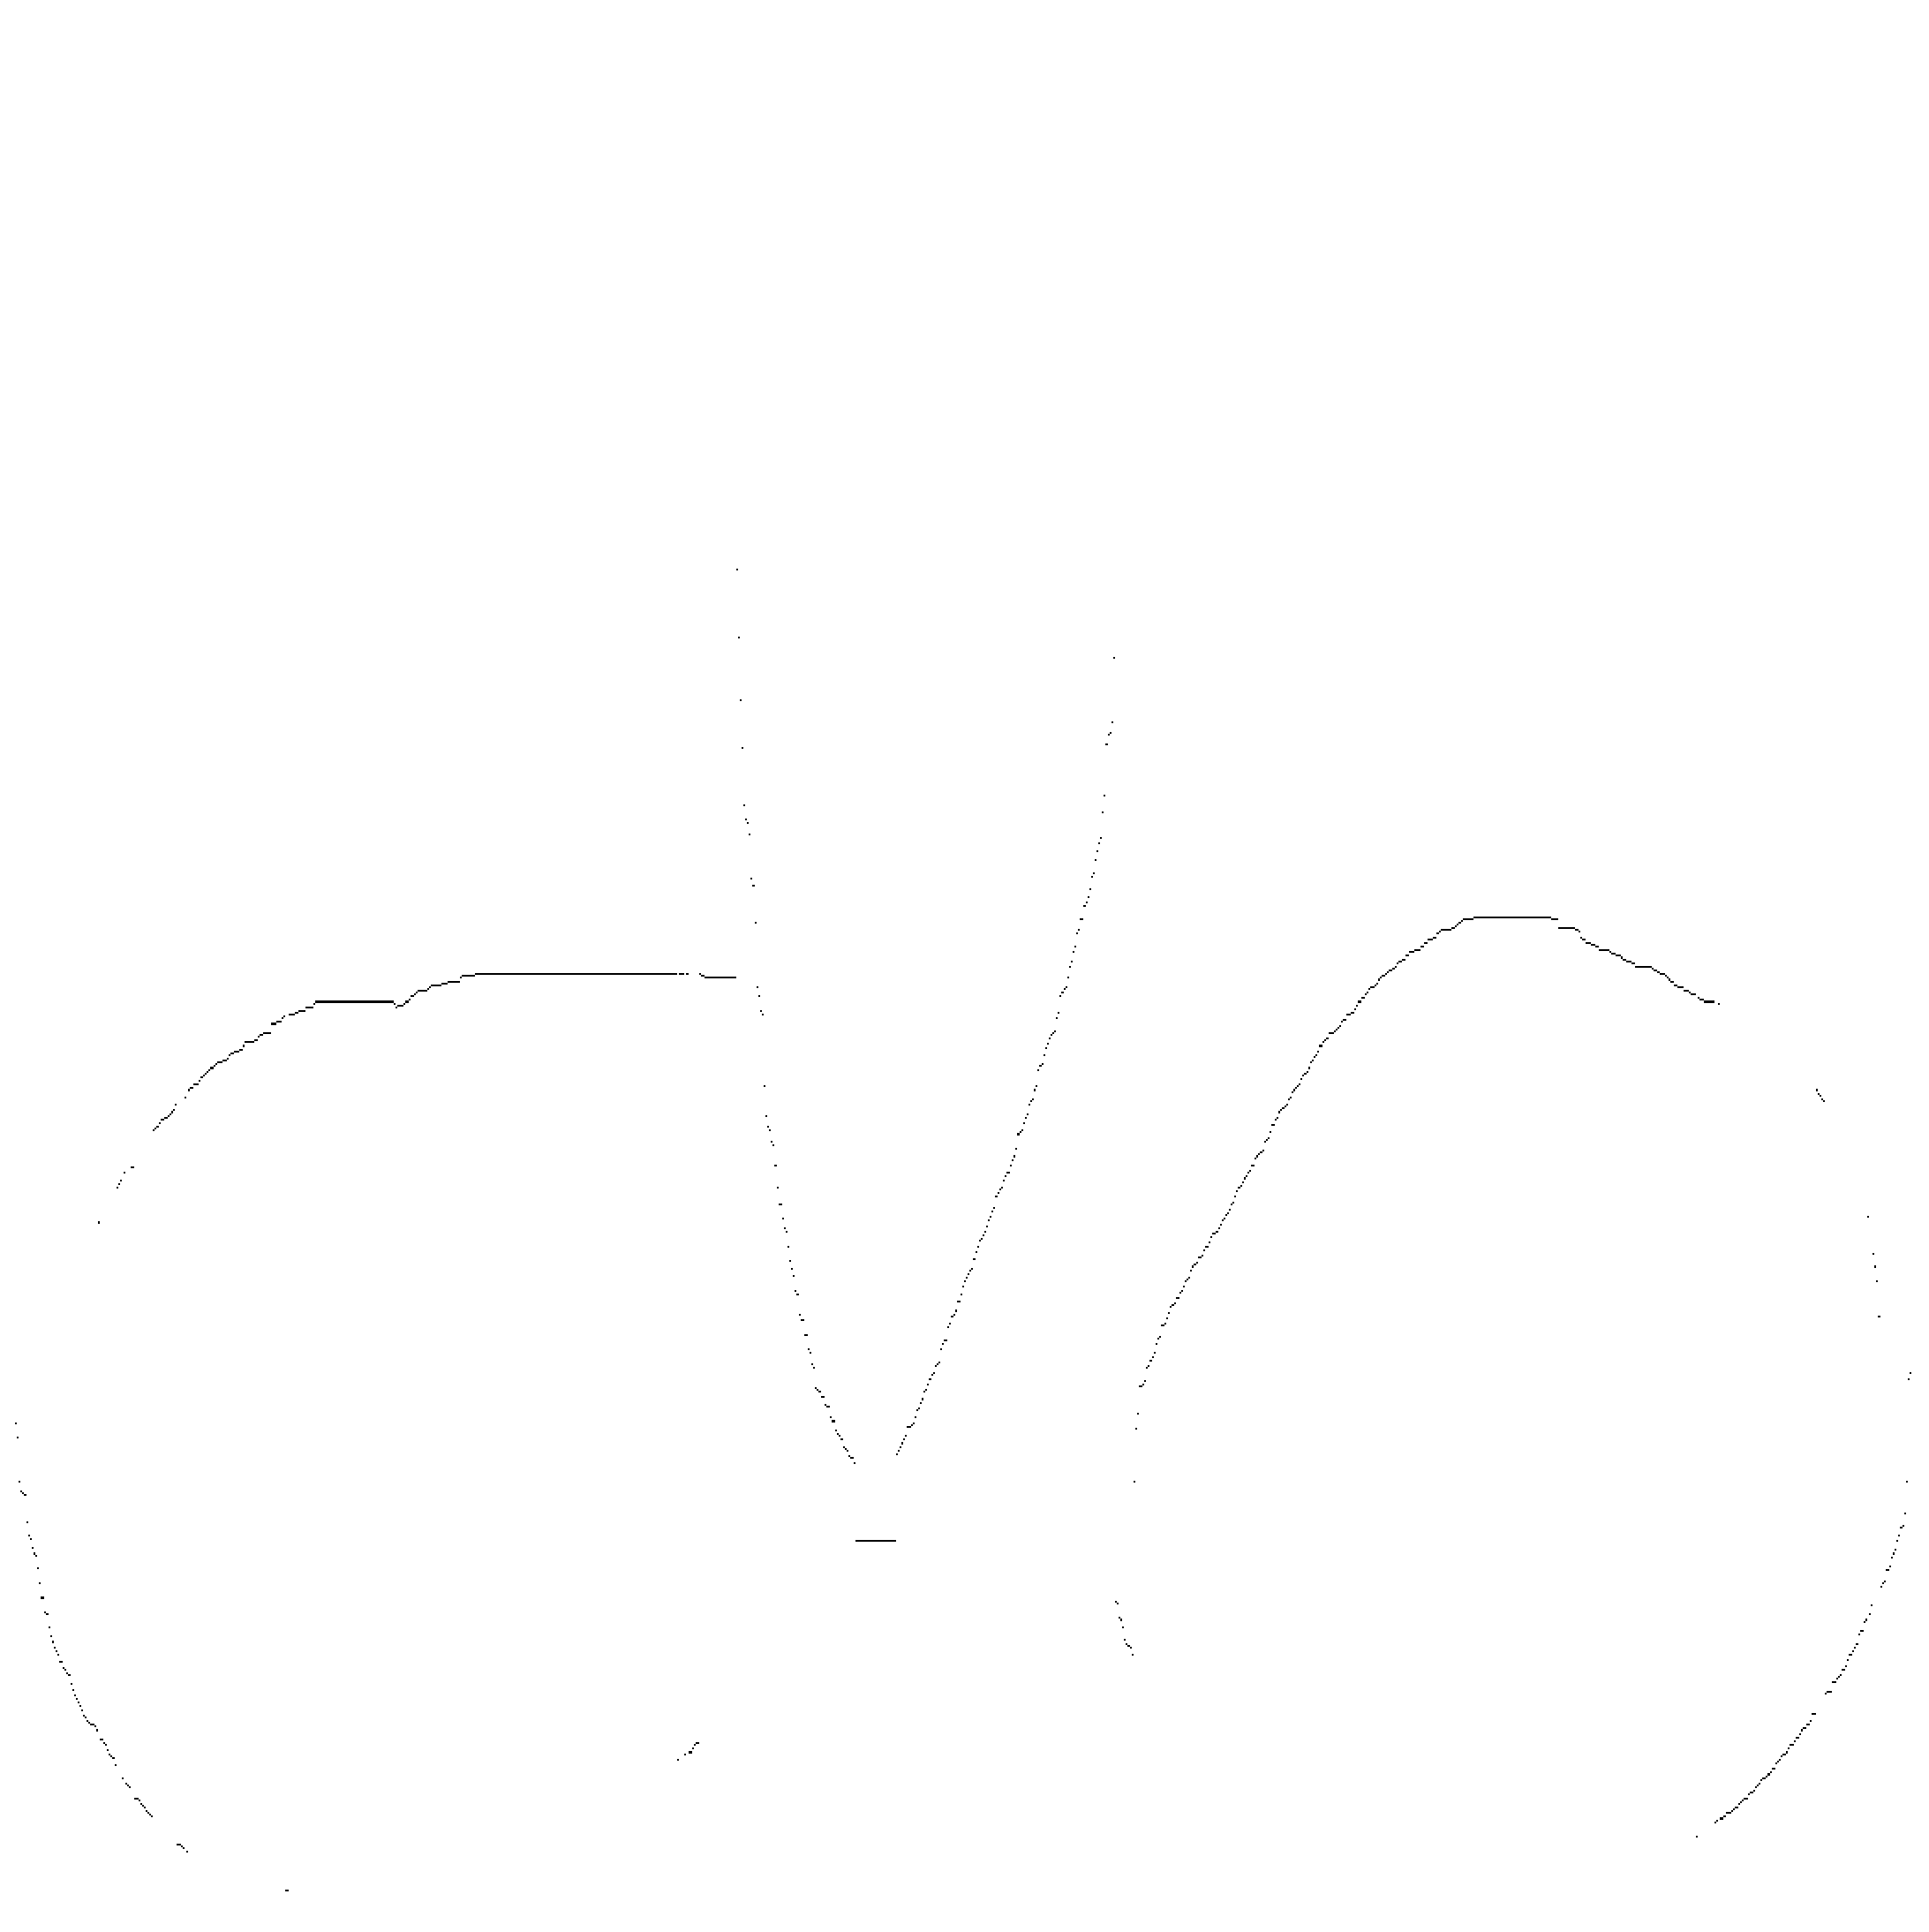
\includegraphics[width=\textwidth]{images/do_lowcont.eps}
\caption{}\label{fig:pasos_mala_seg_inf}
\end{subfigure}
~
\begin{subfigure}[b]{0.25\textwidth}
\centering
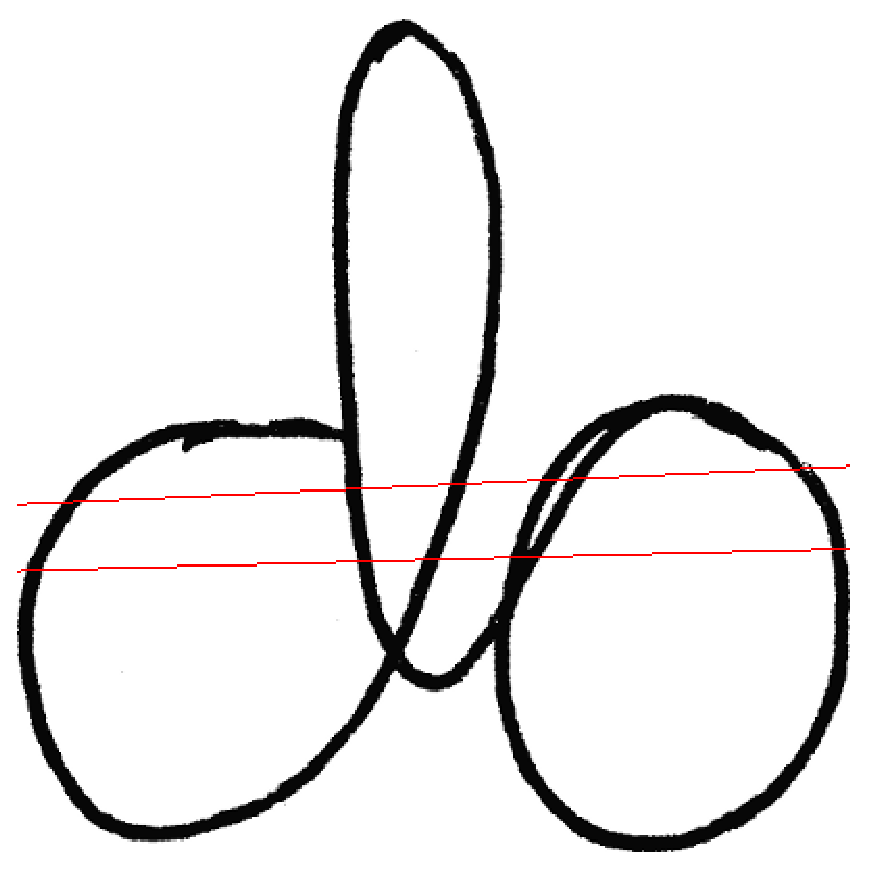
\includegraphics[width=\textwidth]{images/do_result.eps}
\caption{}\label{fig:pasos_mala_seg_lines}
\end{subfigure}
\\
\begin{subfigure}[b]{0.7\textwidth}
\centering
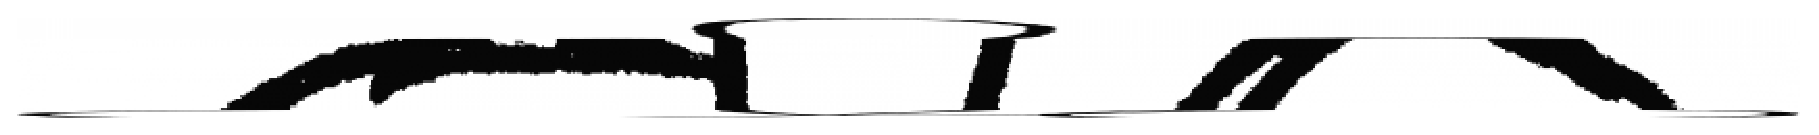
\includegraphics[width=\textwidth]{images/do_norm.eps}
\caption{}\label{fig:pasos_mala_seg_norm}
\end{subfigure}
\caption{Exemple d'una segmentació dolenta i els seus efectes. La figura \ref{fig:pasos_mala_seg_original} mostra la imatge original, la figura \ref{fig:pasos_mala_seg_rlsa} el resultat de l'algorisme RLSA, les figures \ref{fig:pasos_mala_seg_inf} i \ref{fig:pasos_mala_seg_sup} les vores inferior i superior detectades, la \ref{fig:pasos_mala_seg_lines} mostra les línies obtingudes a partir de les vores i finalment la figura \ref{fig:pasos_mala_seg_norm} el resultat de la normalització.}\label{fig:pasos_mala_segmentacio}
\end{figure}

\section{Aproximació utilitzant aprenentatge supervisat}
\label{sec:seg_nn}
Aquesta aproximació a la segmentació del cos central del text que fa ús d'aprenentatge supervisat fou presentada en \cite{DBLP:conf/pris/Gorbe-MoyaEZB08} i fa ús d'una xarxa neuronal multicapa per a classificar certs punts de la imatge en cinc classes: ascendent, línia superior, línia inferior, descendent i altres.\\

Per tal d'utilitzar aquesta tècnica s'han d'extreure un conjunt de punts extrems locals a partir del contorn de la imatge. Aquests punts s'obtenen de la següent manera.
\begin{enumerate}
\item Per a cada columna de la imatge, es busquen els punts de la frontera entre un píxel de fons (típicament blancs) i un píxel d'un símbol (típicament negres). D'aquesta manera s'obté el contorn de la imatge.
\item Els punts seleccionats s'agrupen per línies utilitzant un criteri de proximitat.
\item NO ESTÀ CLAR!
\end{enumerate}

Una vegada s'han obtingut els extrems locals, es situa una finestra de $W_w \times H_w$ píxels centrada en cada punt. Aquesta finestra es redueix a una grandària de $W_f \times H_f$ utilitzant una distorsió d'ull de peix, de manera que els punts a prop del lloc d'interés queden ressaltats sobre aquells més llunyans. Aquesta serà l'entrada a la xarxa neuronal.\\

Per a entrenar la xarxa neuronal, s'utilitzen imatges amb els seus extrems locals classificats manualment, de manera que la xarxa neuronal aprèn a classificar un extrem local en una de les cinc classes mencionades anteriorment. Alternativament, per a facilitar l'entrenament del sistema, un humà pot corregir els punts classificats automàticament per un altre sistema més rudimentari per a la detecció de les línies de referència \cite{DBLP:conf/pris/Gorbe-MoyaEZB08}. Els detalls sobre l'entrenament de xarxes neuronals poden consultar-se en diverses fonts sobre aprenentatge automàtic \cite{DH73,bishop2006pattern,murphy2012machine}.

Per a segmentar el cos central d'una imatge de \emph{test}, es classifiquen tots els punts utilitzant la xarxa neuronal entrenada anteriorment. Llavors tots els punts pertanyents a una mateixa classe són utilitzats per a fer una interpolació lineal i obtenir cadascuna de les quatre línies de referència (els píxels classificats com ``altres'' no s'utilitzen).\\

La figura \ref{fig:comp_seg_mlp_result} mostra el resultat d'aplicar l'anterior algorisme a una imatge que conté text manuscrit. Els punts marcats són els extrems locals classificats, les línies verdes són la línia base superior i inferior i les roges marquen el l'altura dels ascendents i descendents.\\

% COMPARACIÓ VISUAL ENTRE LES DUES TÈCNIQUES
\begin{figure}
\centering
\begin{subfigure}[b]{0.9\textwidth}
\centering
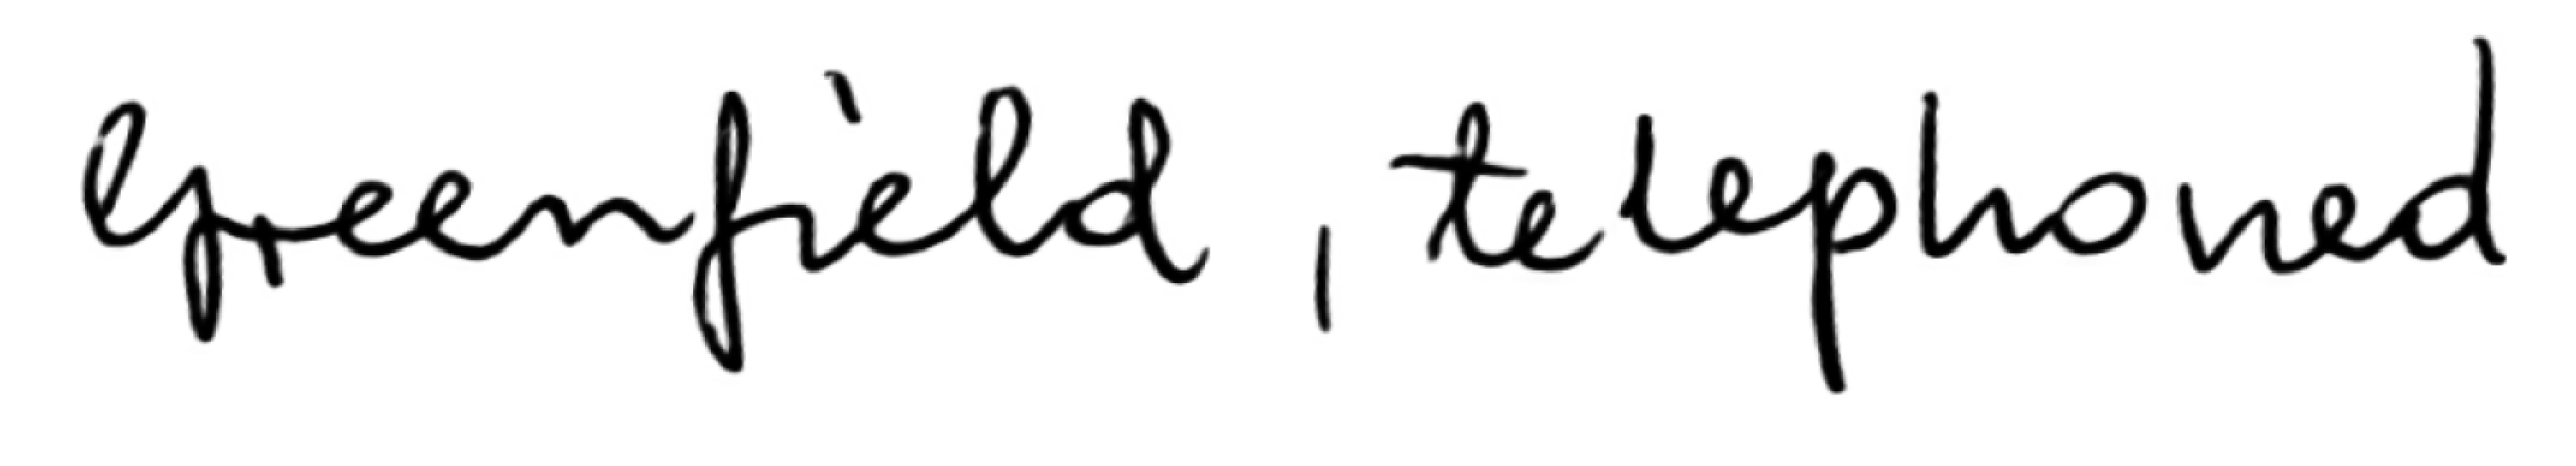
\includegraphics[width=\textwidth]{images/comp_seg_original.eps}
\caption{}\label{fig:comp_seg_original}
\end{subfigure}\\
% Resultat de la segmentació segons cada tècnica.
\begin{subfigure}[b]{0.9\textwidth}
\centering
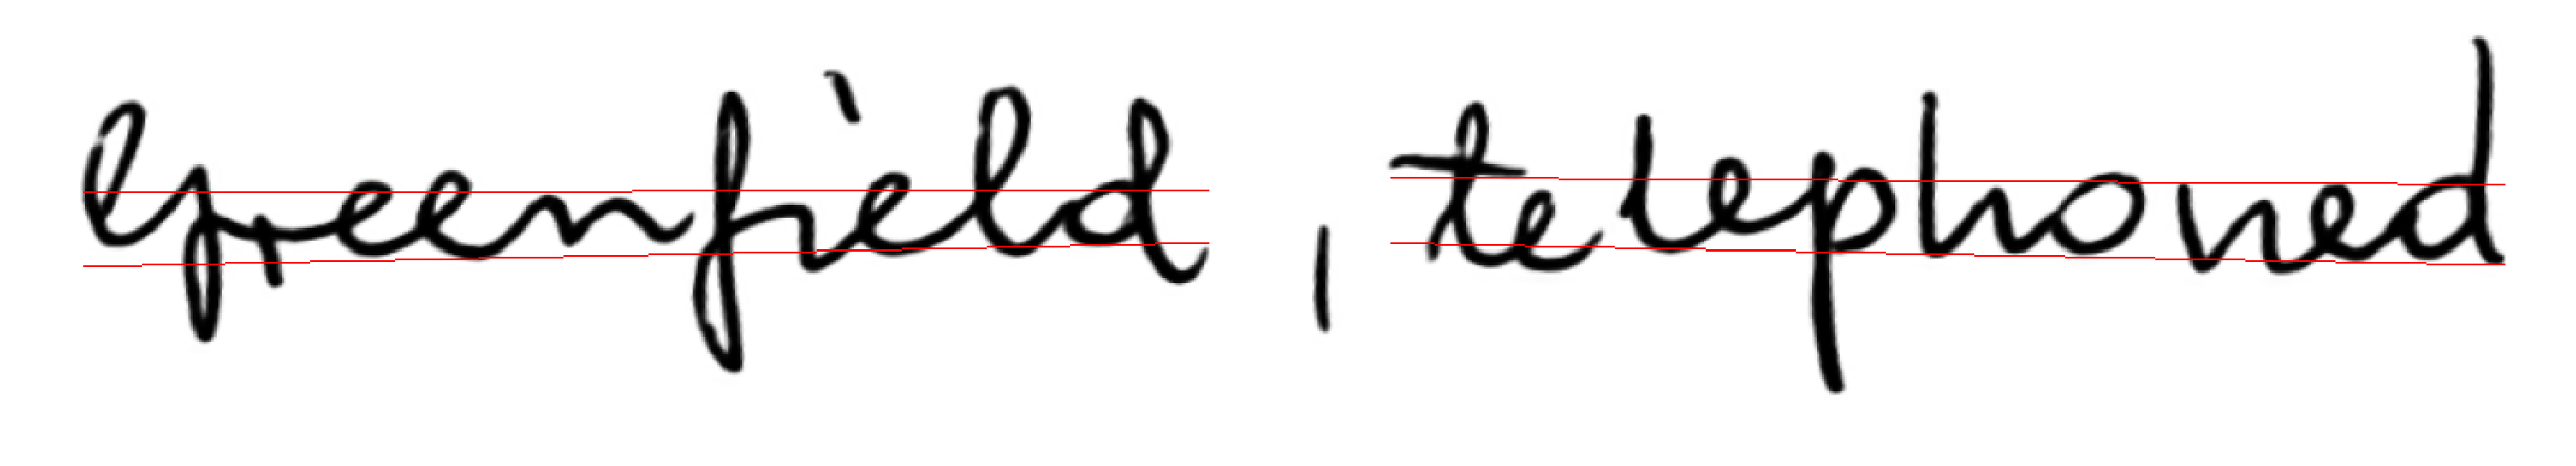
\includegraphics[width=\textwidth]{images/comp_seg_heur_result.eps}
\caption{}\label{fig:comp_seg_heur_result}
\end{subfigure}\\
\begin{subfigure}[b]{0.9\textwidth}
\centering
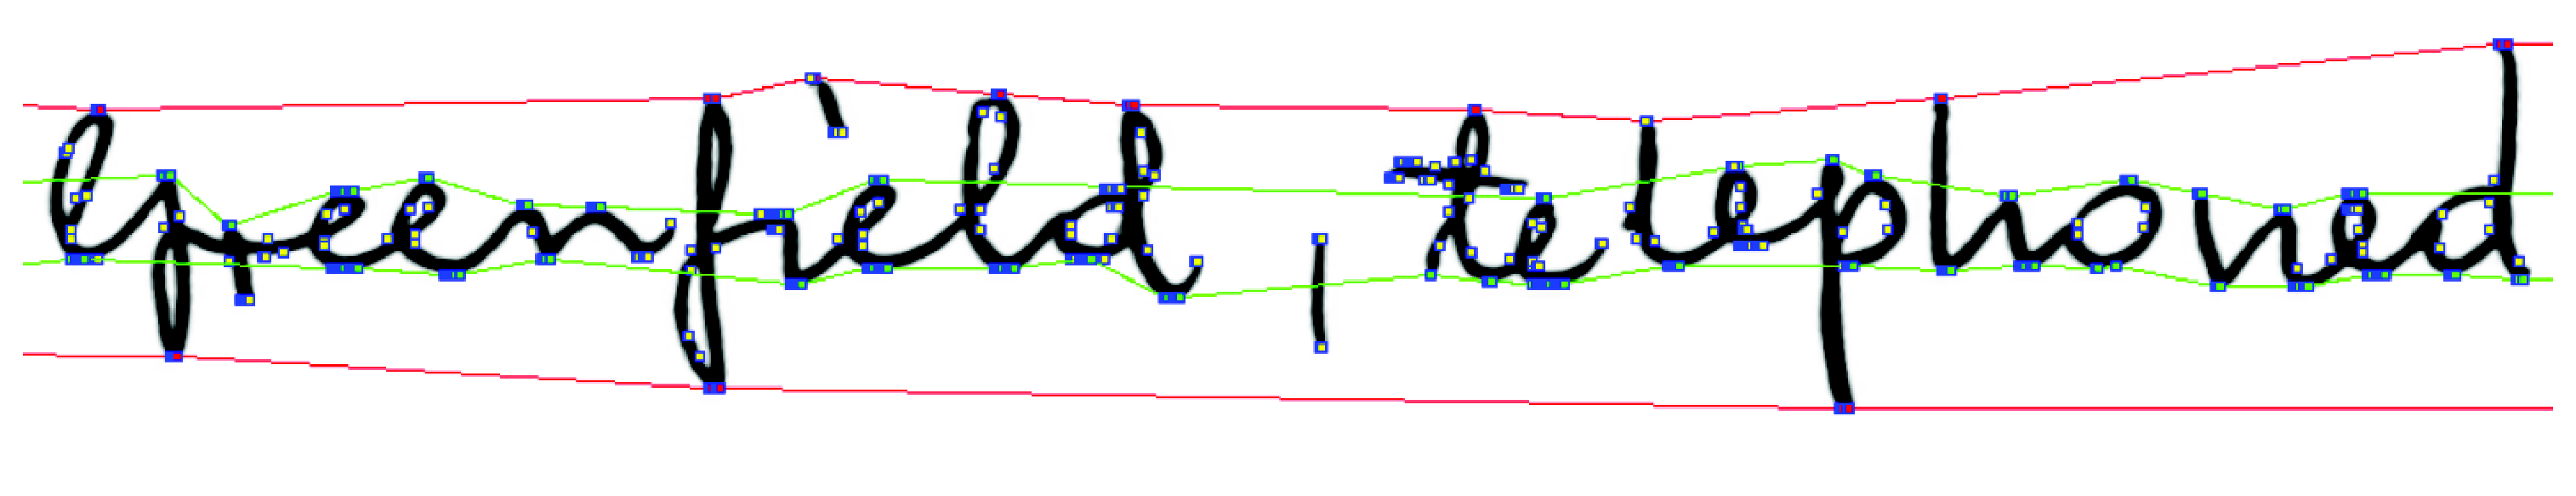
\includegraphics[width=\textwidth]{images/comp_seg_mlp_result.eps}
\caption{}\label{fig:comp_seg_mlp_result}
\end{subfigure}\\
% Resultat de la normalització segons cada tècnica.
\begin{subfigure}[b]{0.9\textwidth}
\centering
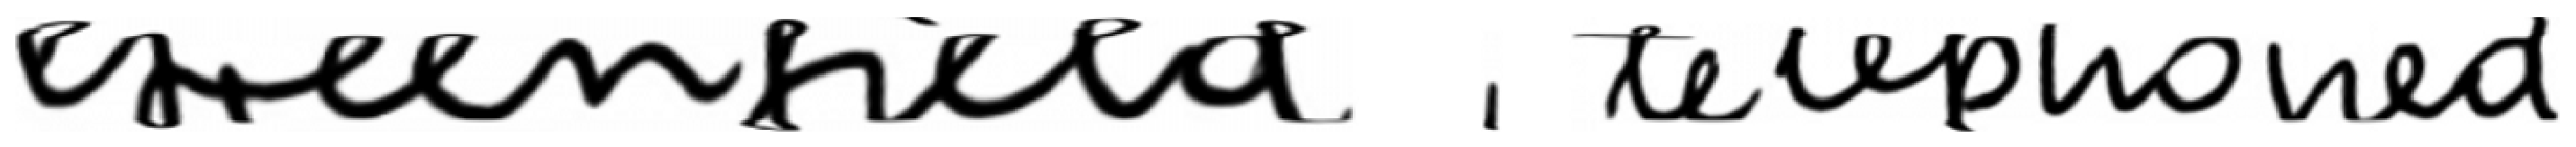
\includegraphics[width=\textwidth]{images/comp_seg_heur_norm.eps}
\caption{}\label{fig:comp_seg_heur_norm}
\end{subfigure}\\
\begin{subfigure}[b]{0.9\textwidth}
\centering
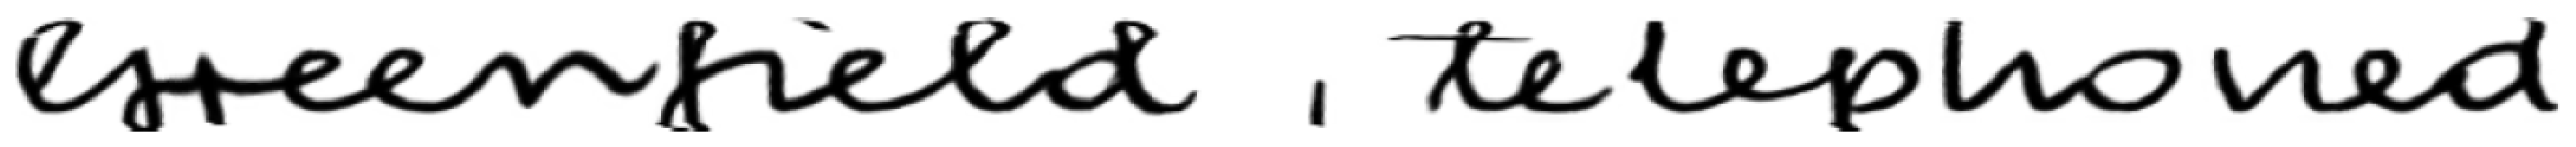
\includegraphics[width=\textwidth]{images/comp_seg_mlp_norm.eps}
\caption{}\label{fig:comp_seg_mlp_norm}
\end{subfigure}
\caption{Imatge original (\ref{fig:comp_seg_original}), segmentació del cos central segons l'aproximació heurística i basada en aprenentatge supervisat (\ref{fig:comp_seg_heur_result}, \ref{fig:comp_seg_mlp_result}) i resultat de la normalització segons cada aproximació (\ref{fig:comp_seg_heur_norm}, \ref{fig:comp_seg_mlp_norm}) \cite{DBLP:conf/pris/Gorbe-MoyaEZB08}.}\label{fig:comp_seg}
\end{figure}

Les figures \ref{fig:comp_seg_heur_result} i \ref{fig:comp_seg_mlp_result} mostren les diferències en les assumpcions que fan cadascun dels dos mètodes explicats. La major informació que aporta la detecció de les línies de referència utilitzant el mètode supervisat pot oferir clarament una millora significativa a l'hora d'aplicar el procés de normalització a la imatge. En els següents capítols s'explicarà com s'han quantificat aquestes diferències per demostrar que, efectivament, l'ús del mètode supervisat millora considerablement el reconeixement de text manuscrit.